\section{Results}
\label{sec:result}

\begin{figure*}[t]
\centering
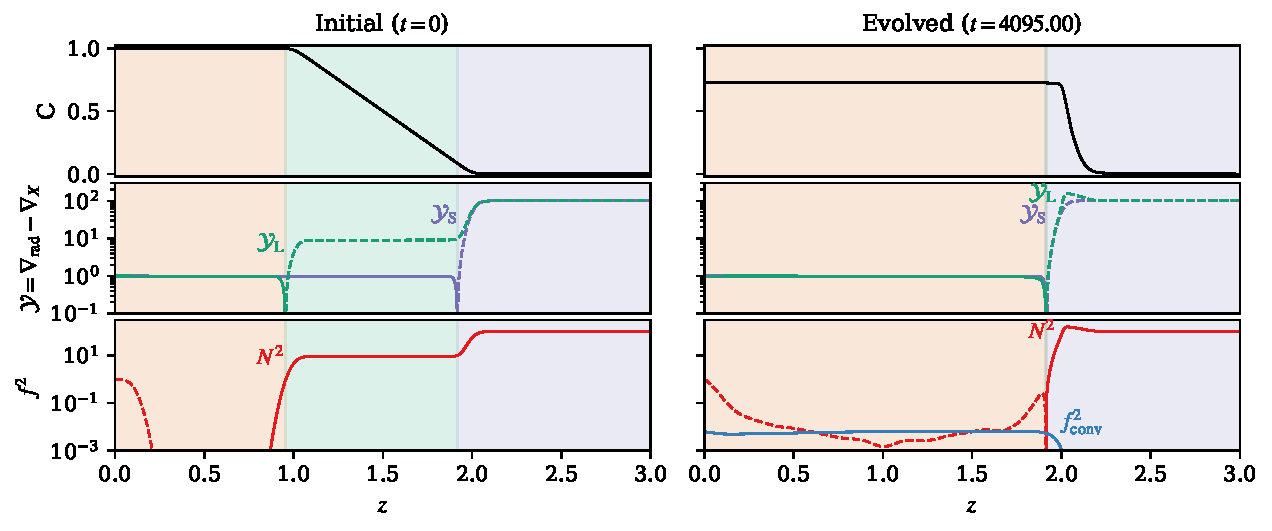
\includegraphics[width=\textwidth]{fig2_profiles.pdf}
\caption{
\label{fig:profiles}
}
\end{figure*}



\begin{itemize}
\item We simulate a three-layer system with X properties using the Dedalus pseudospectral solver.
We refer the reader to appendices~\ref{app:model} and \ref{app:simulation_details} for details of the model assumptions, setup, and numerical methods.
\item In figure \ref{fig:dynamics} we show volume visualizations of instantaneous dynamics near the beginning, during the entrainment phase, and in the evolved state of one of these simulations.
Here is a description of the things to look for in these visualizations.
I should write this before I decide which things to put into this figure.
\item In figure \ref{fig:profiles} we show horizontally- and time-averaged profiles of the initial state of the simulation, during the entrainment phase, and in the evolved state.
Here's an in-depth description of what's plotted.
Here's what you should take away from each panel of the plots.
\item In figure \ref{fig:kippenhahn}, we plot a Kippenhahn-like diagram of the simulation.
The orange region is the convection zone, the green region is Ledoux-stable but Schwarzschild-unstable, and the purple region is both Schwarzschild and Ledoux stable.
The line at the top of the orange region determines the boundary of the convection zone according to $y_L$, and the line at the bottom of the purple region determines the CZ boundary according to $y_S$.
While these lines start at different heights, convection entrains low-composition fluid according to a classic $\sqrt{t}$ entrainment law until these criteria are the same.
\end{itemize}

\begin{figure}[t]
\centering
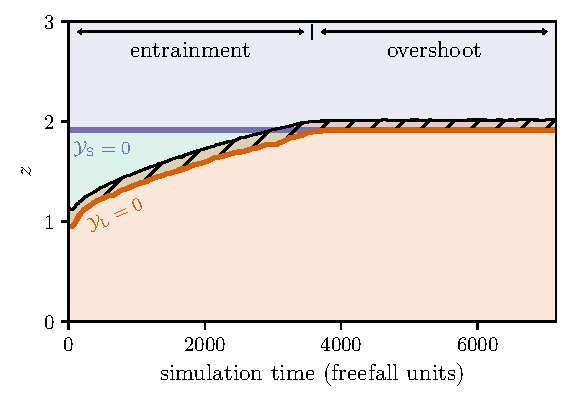
\includegraphics[width=\columnwidth]{kippenhahn.pdf}
\caption{
\label{fig:kippenhahn}
}
\end{figure}


